\definecolor{commentgreen}{RGB}{2,112,10}
\definecolor{eminence}{RGB}{187,0,255}
\definecolor{weborange}{RGB}{255,165,0}
\definecolor{frenchplum}{RGB}{129,20,83}

\lstset{
  basicstyle=\ttfamily\footnotesize\linespread{1.2}\selectfont,
  numbers=left,
  language=C,
  numberstyle=\tiny,
  breaklines=true,
    xleftmargin=2em,
  escapeinside={(*@}{@*)},
  commentstyle=\color{commentgreen},
keywordstyle=\color{eminence},
stringstyle=\color{red},
emph={int,char,double,float,unsigned,void,bool},
    emphstyle={\color{blue}},
}

\section{Implementation der Algorithmen}

Im Folgenden sind die verwendeten Speicherverhaltungsalgorithmen dargestellt.

\subsection{first fit}

\begin{lstlisting}[caption={first fit C-Implementation}, label=listing:firstFit]
unsigned firstFitAlloc(unsigned blockSize) {
  unsigned address = 0;

  // loop over free space to check if there is a block bigger than blockSize
  for (unsigned i = 0; i < freeList.size(); i++) {
    if (freeList[i].size >= blockSize) {
      // free space found
      address = allocBlock(i, blockSize);
      break;
    }
  }

  return address;
}
\end{lstlisting}

Bei first-fit wird der erste verfügbare Speicherblock verwendet. Dazu wird in der Implementation \ref{listing:firstFit} über den Vektor \textit{freeList} iteriert. Wird ein Block gefunden, welcher gleich groß oder größer ist, wird dieser alloziert und die Suche abgebrochen.

\subsection{next fit}

\begin{lstlisting}[caption={next fit C-Implementation}, label=listing:nextFit]
unsigned nextFitAlloc(unsigned blockSize) {
  unsigned lastAddressNextFit = 0; 
  unsigned address = 0;

  if (freeList.empty())
    return address;

  if (lastAddressNextFit == 0) {
    lastAddressNextFit = freeList.front().address;
  }

  // search for lastAddressNextFit
  unsigned lastAddress_idx = 0;
  for (unsigned i = 0; i < freeList.size()-1; i++) {
    if (freeList[i].address >= lastAddressNextFit && lastAddressNextFit <= freeList[i+1].address) {
      lastAddress_idx = i;
      break;
    }
  }

  // loop over free space to check if there is a block bigger than blockSize
  // start at last Address
  unsigned n = freeList.size();
  for (unsigned j = 0; j < n; j++) {
    unsigned i = (lastAddress_idx + j) % n;
    if (freeList[i].size >= blockSize) {
      lastAddressNextFit = freeList[i].address;
      address = allocBlock(i, blockSize);
      break;
    }
  }
  if (address == 0)
    lastAddressNextFit = 0;

  return address;
}
\end{lstlisting}

Next-fit funktioniert wie first-fit. Der Unterschied ist, dass next-fit die letzte allozierte Adresse speichert und diese als Startpunkt der first-fit Suche verwendet. In der Implementation von next-fit \ref{listing:nextFit} wird dies über die globale Variable \text{lastAddressNextFit} realisiert. Es wurde sich für die Speicherung der Adresse und nicht des letzte Indexes entschieden, da der Index innerhalb des Vektors durch die zufällige freigabe von Speicherblöcken verändern kann.

Daher wird in den Zeilen 11 bis 17 die Addresse in einen Index umgewandelt. Da sich durch die vorherige Allozierung die Adressen in \textit{freeList} ändern, wird nach einer passenden Lücke für die alte Adresse gesucht. Anschließend wird der nächste freie Block in dem Vektor \textit{freeList} gesucht und alloziert. Über die Rechenvorschrift \textit{(lastAdress\_idx + j) \% n} wird dafür gesorgt, dass die Suche bei \textit{lastAdress\_idx} startet und wieder endet.


\subsection{best fit}

\begin{lstlisting}[caption={best fit C-Implementation}, label=listing:bestFit]
unsigned bestFitAlloc(unsigned blockSize) {
  unsigned address = 0;

  // loop over free space to find smallest fitting block
  int best = -1;
  unsigned lastFit = UINT_MAX;
  for (unsigned i = 0; i < freeList.size(); i++) {
    int nextFit = freeList[i].size - blockSize;
    if (nextFit >= 0 && (unsigned)nextFit < lastFit) {
      best = i;
      lastFit = nextFit;
    }
  }
  if (best == -1)
    return 0;
  address = allocBlock(best, blockSize);

  return address;
}
\end{lstlisting}

Best-Fit sucht einen freien Speicherblock, welcher nach allozieren den kleinsten neuen Speicherblock erzeugt. Die Implementation \ref{listing:bestFit} erreicht dies durch eine Suche über \textit{freeList}. Bei jedem Element wird verglichen, ob der Speicherblock groß genug ist und ob der überbleibende Block kleiner ist, als der letzte beste Wert. Anschließend wird der gefundene Block alloziert.

\subsection{worst fit}

\begin{lstlisting}[caption={worst fit C-Implementation}, label=listing:worstFit]
unsigned worstFitAlloc(unsigned blockSize) {
  unsigned address = 0;

  // loop over free space to find biggest fitting block
  int best = -1;
  unsigned lastFit = 0;
  for (unsigned i = 0; i < freeList.size(); i++) {
    int nextFit = freeList[i].size - blockSize;
    if (nextFit >= 0 && (unsigned)nextFit > lastFit) {
      best = i;
      lastFit = nextFit;
    }
  }
  if (best == -1)
    return 0;
  address = allocBlock(best, blockSize);

  return address;
}
\end{lstlisting}

Worst-Fit sucht einen freien Speicherblock, welcher nach allozieren den größten neuen Speicherblock erzeugt. Die Implementation \ref{listing:worstFit} ist gleich der implementation von best-fit \ref{listing:bestFit} mit dem Unterschied, dass die Suchbedingung größere überbleibende Blöcke bevorzugt.

\section{Vergleich}

In \cref{fig:loglog} und \cref{fig:zoom} sind die Ergebnisse vom Test der Algorithmen dargestellt.

Im Vergleich der Algorithmen ist zu erkennen, dass first-fit, next-fit und best-fit ähnliche Ergebnisse liefern. Worst-fit ist der einzige Algorithmus, welcher schlechter abschneidet, als die anderen.

In \cref{fig:best_algo} wurde zusätzlich zur maximalen Größe einer einzelnen Allozierung auch der verfügbare Speicher variiert. Es ist zu erkennen, das best-fit in den meisten Fällen der beste Algorithmus ist. Best-fit ist in 11113 Kombinationen der beste Algorithmus. Am schlechtesten schneidet next-fit mit einem Wert von 684 ab. First-fit und worst-fit schneiden ähnlich mit 1659 und 993 Kombinationen etwas besser als next-fit ab. Die weiße Fläche stellt alle Kombinationen dar, in denen es mehr als zwei beste Algorithmen gibt und dominiert mit 25152 Kombinationen.
Die Transparenz gibt an, wie knapp ein Algorithmus gewonnen hat. Dadurch ist zu erkennen, dass bei einem Verhältnis von kleiner Allozierungröße und großem vorhandenen Speicher best-fit Mit einem größeren Abstand der beste Algorithmus ist.

Es ist zu erwarten, dass first-fit und next-fit ähnliche Werte erreichen, da sie ähnlich Implementationen haben. Worst-fit schneidet am schlechtesten ab.

\cref{fig:time} vergleicht die benötigte Zeit von jedem Algorithmus zu den erreichten maximalen Allozierungen. Dabei ist zu erkennen, dass worst-fits Ziel vom reduzieren der Zeit im Vergleich zu best-fit klappt. First-fit hingegen erreicht fast so viele Allozierungen, wie best-fit, in einer geringeren Zeit.

\begin{figure}
  \center
  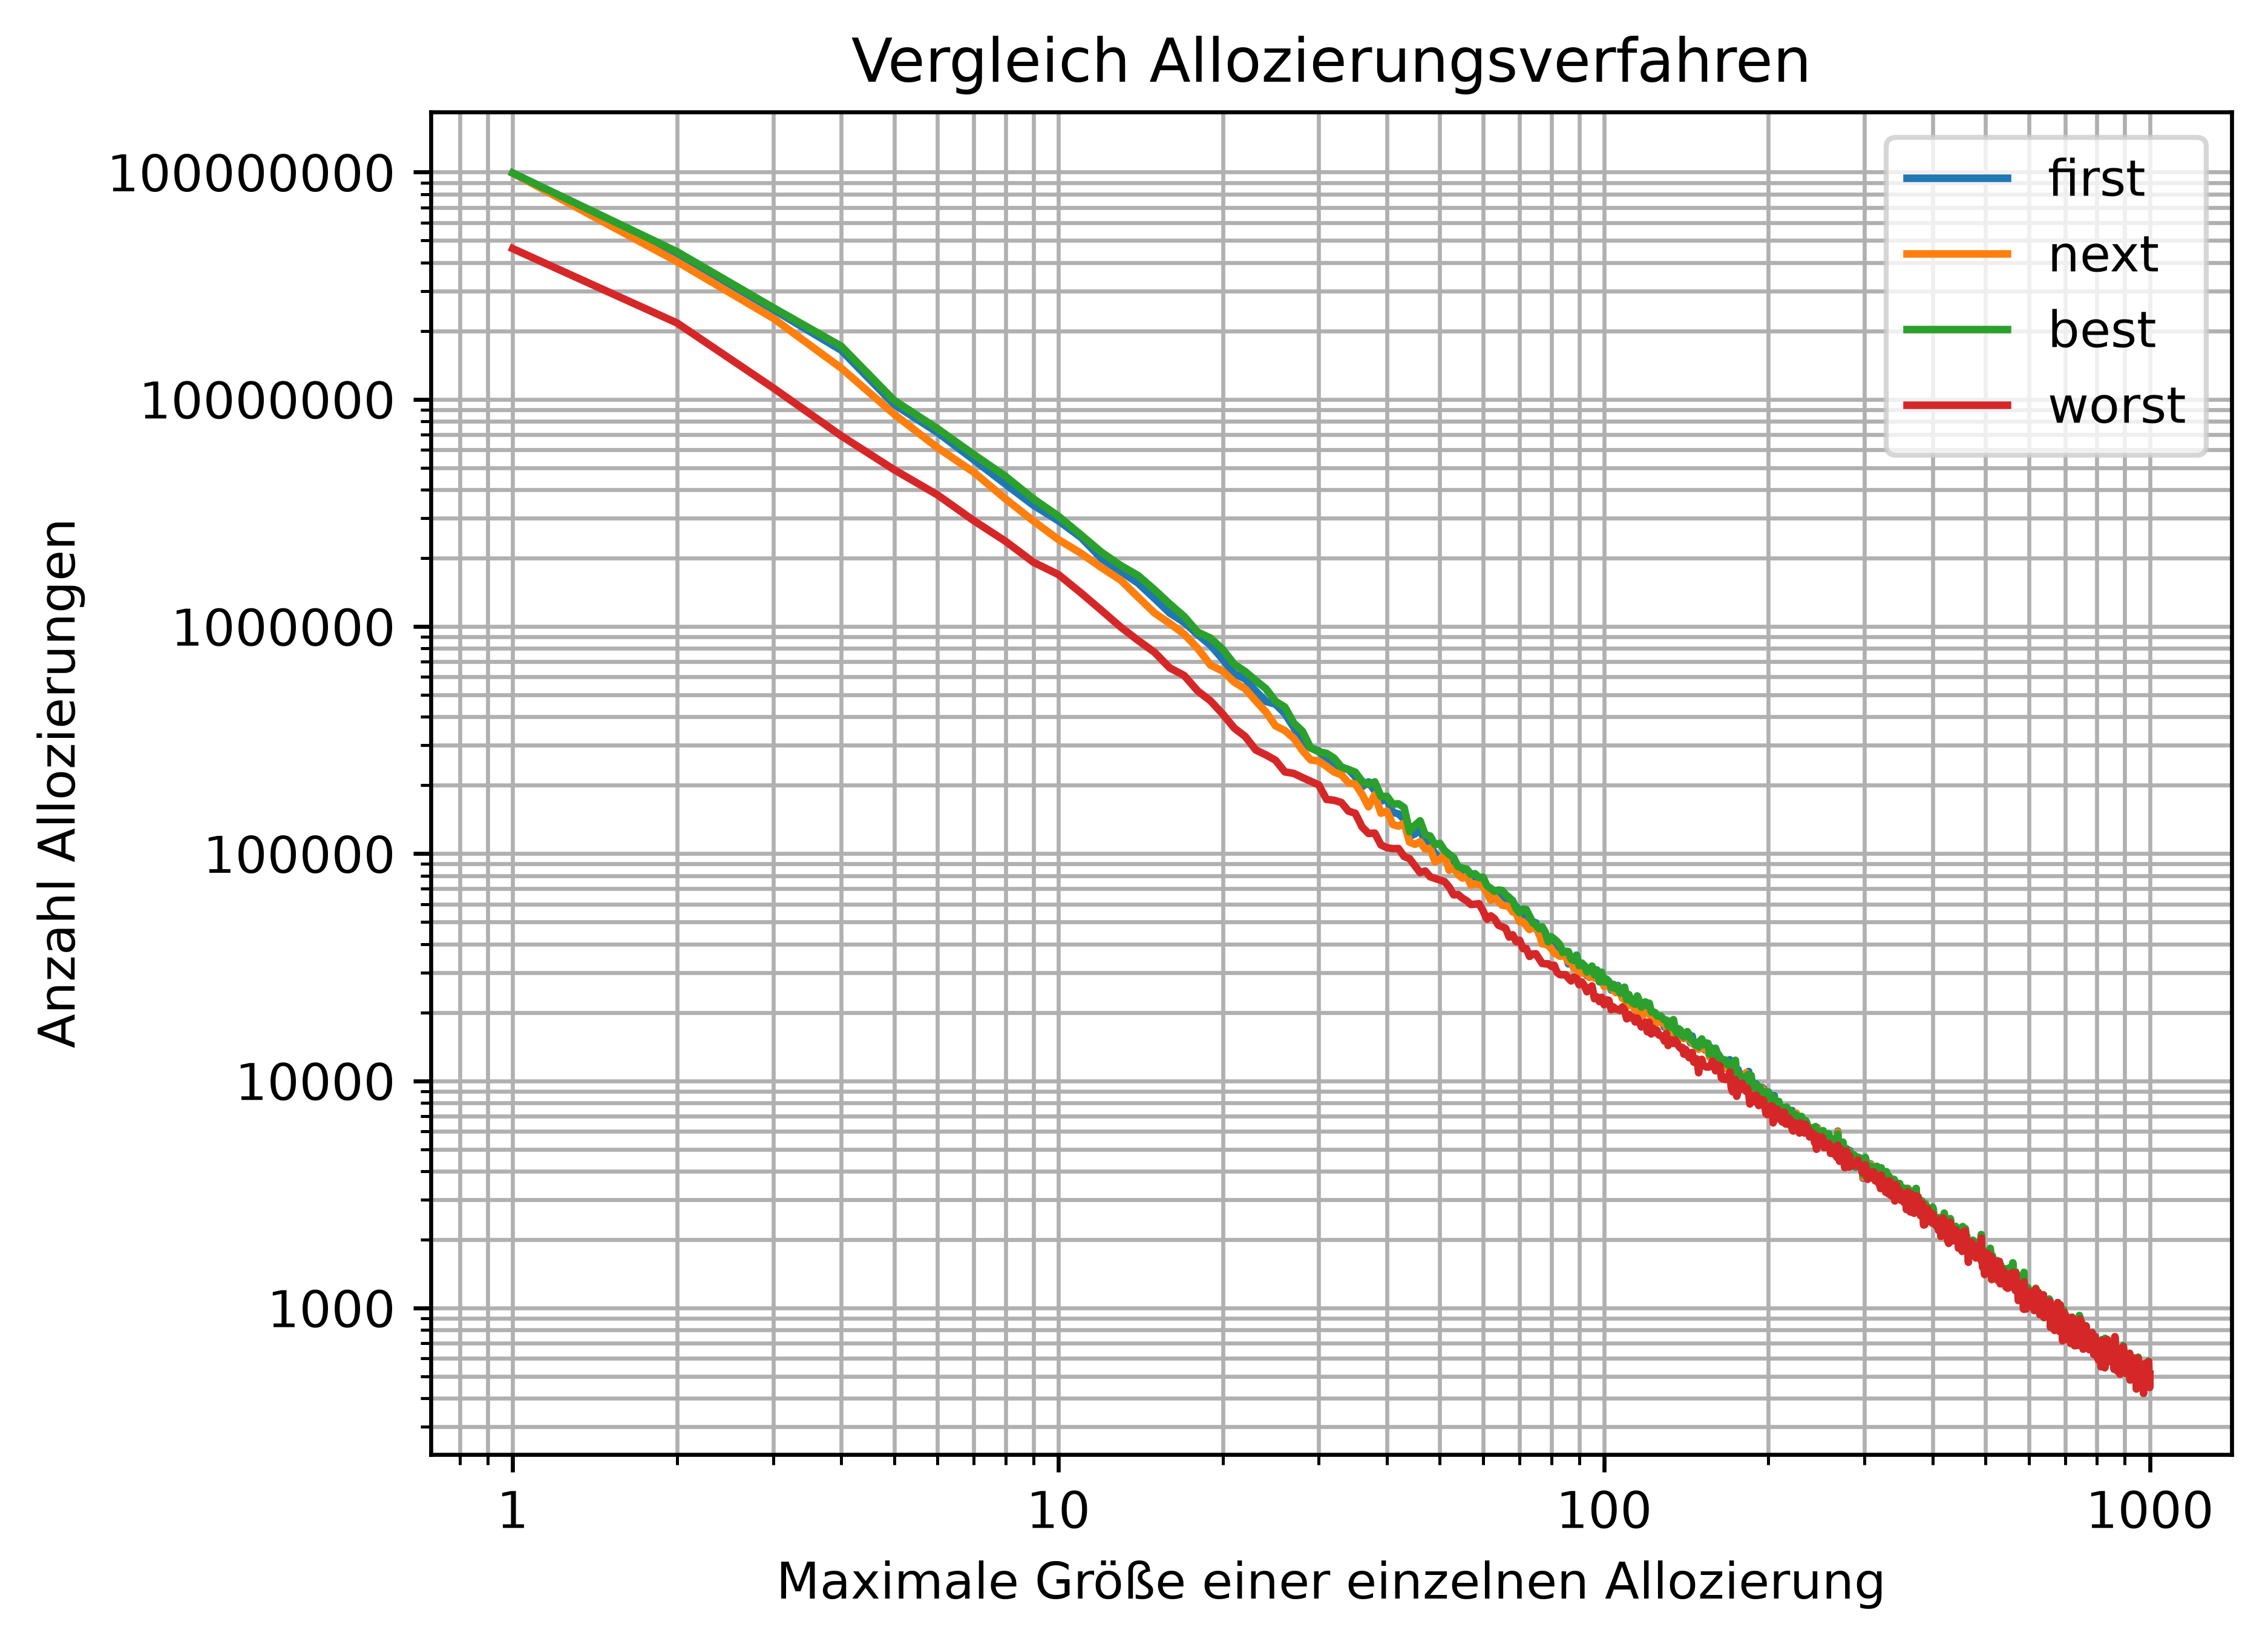
\includegraphics[width=.7\textwidth]{images/vergleich_loglog.png}
  \caption{Vergleich Algorithmen in loglog Darstellung.}
  \label{fig:loglog}
\end{figure}

\begin{figure}
  \center
  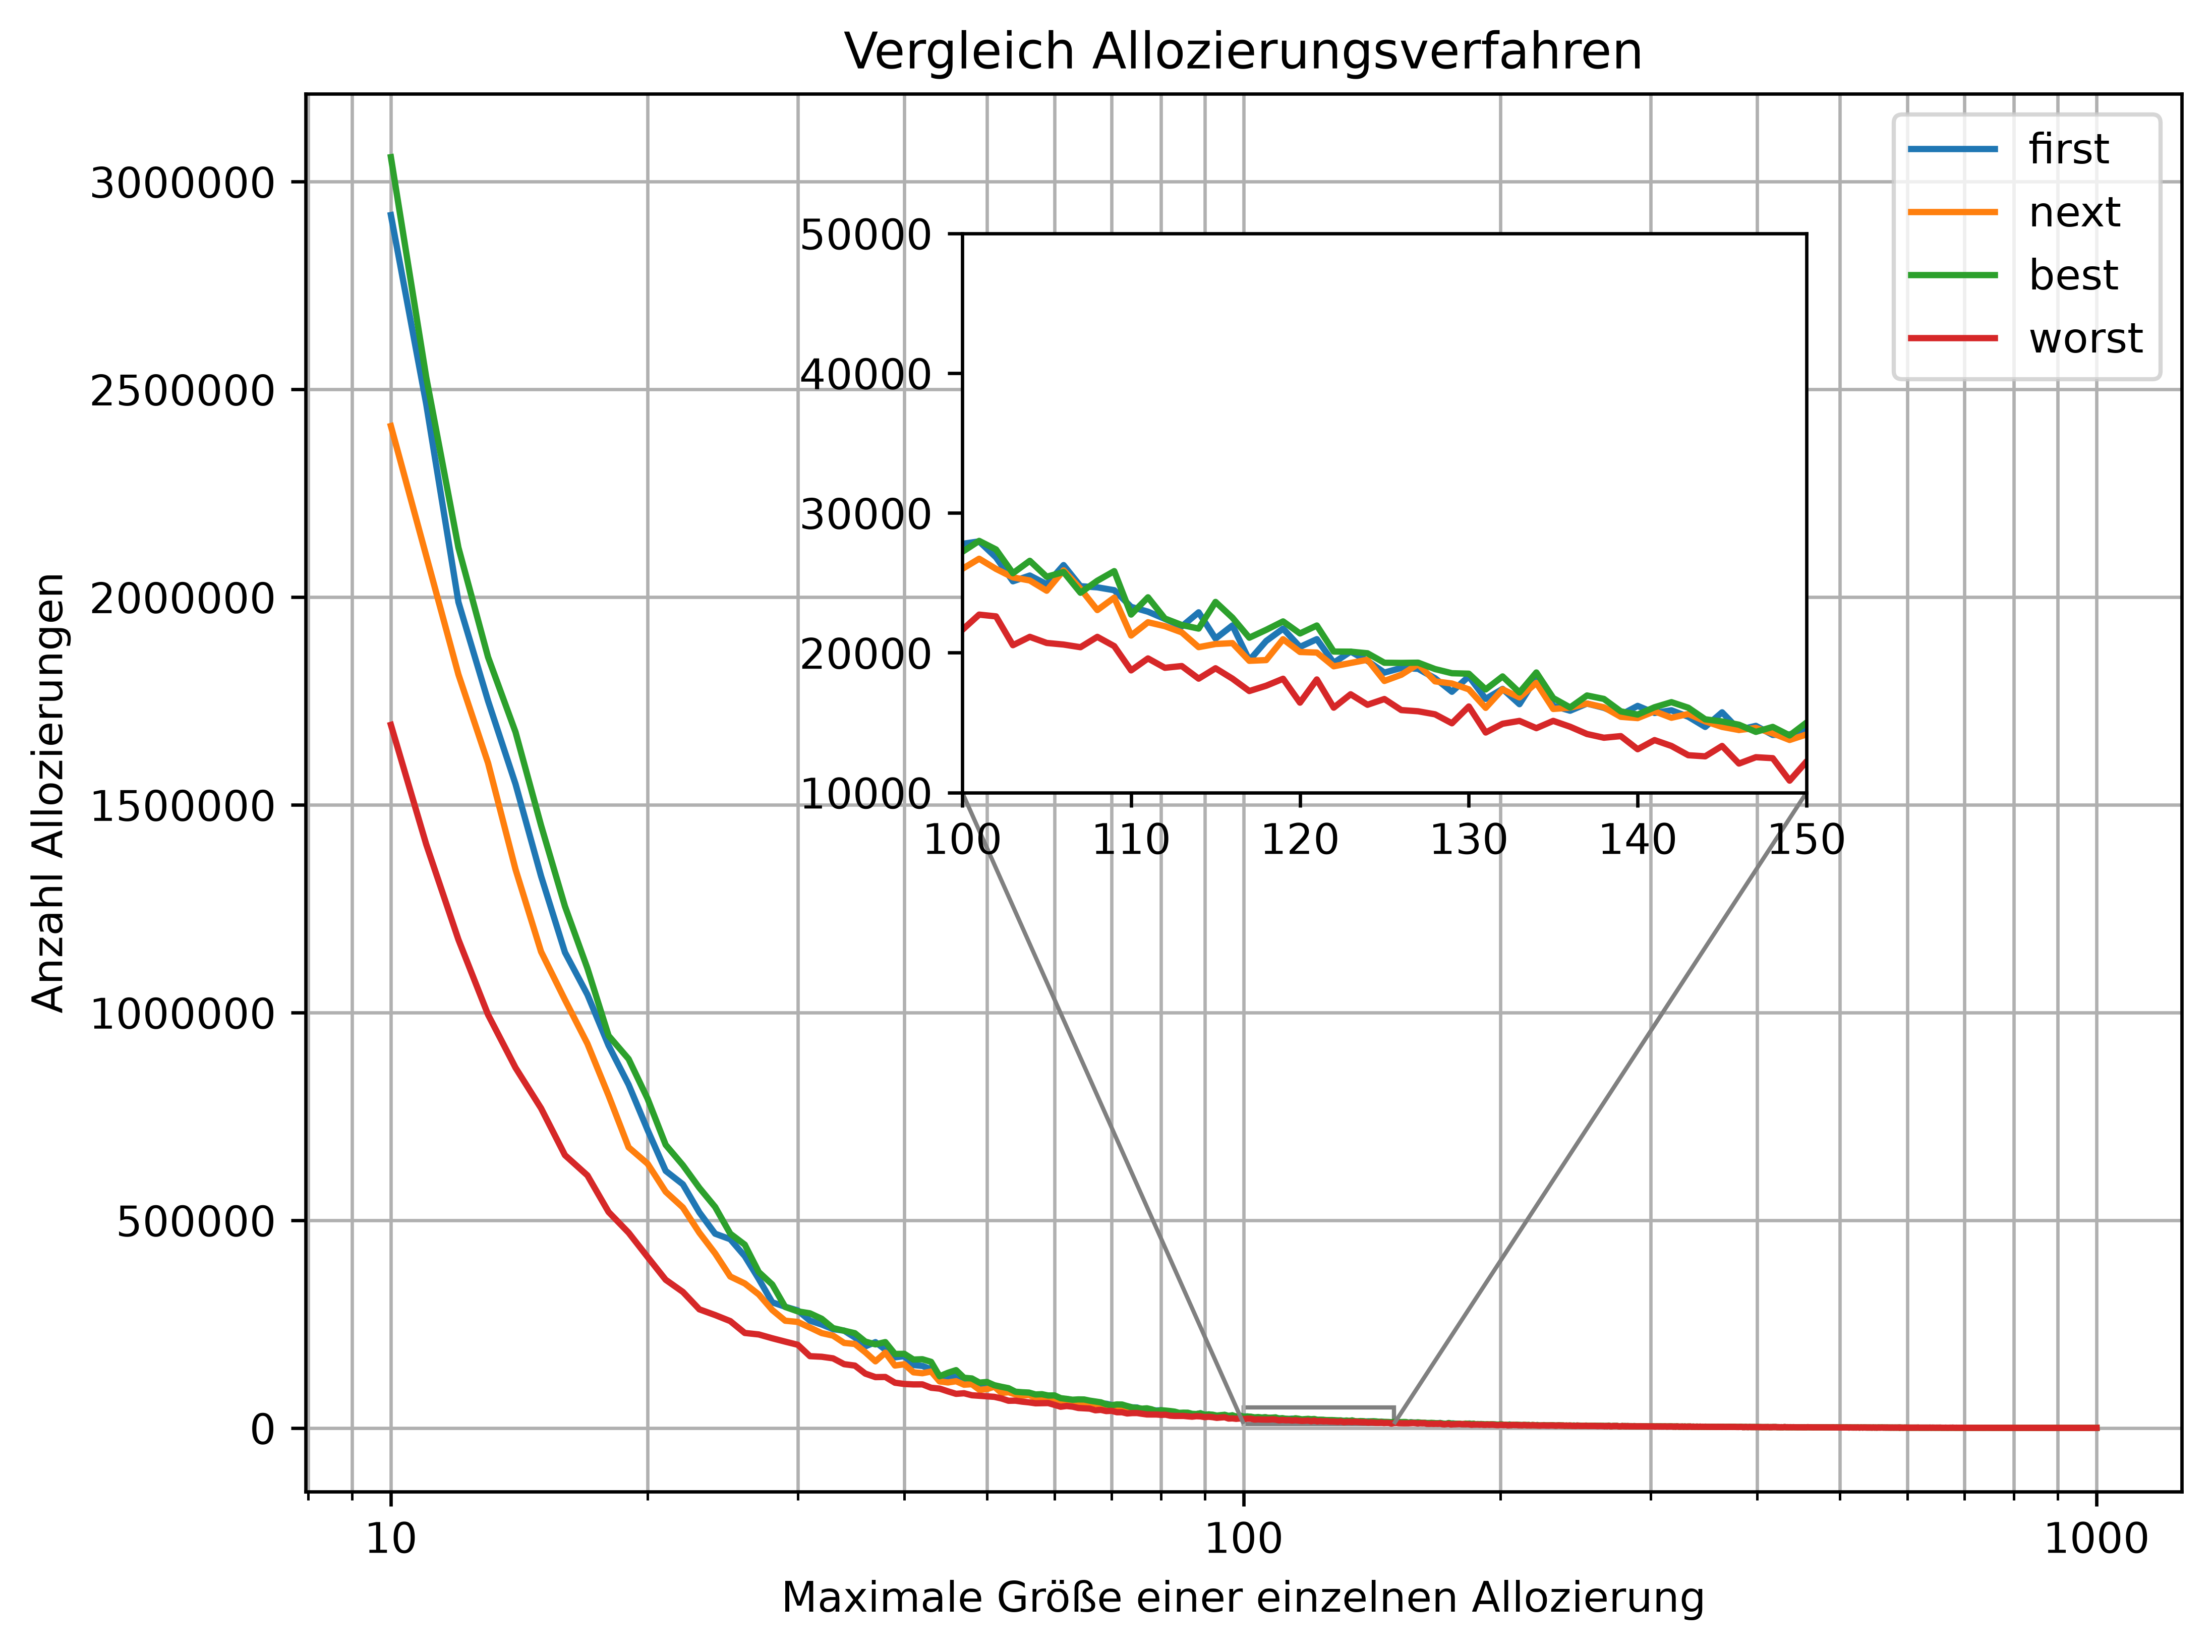
\includegraphics[width=.7\textwidth]{images/vergleich_zoom.png}
  \caption{Vergleich Algorithmen in einfacher log Darstellung.}
  \label{fig:zoom}
\end{figure}

\begin{figure}
  \center
  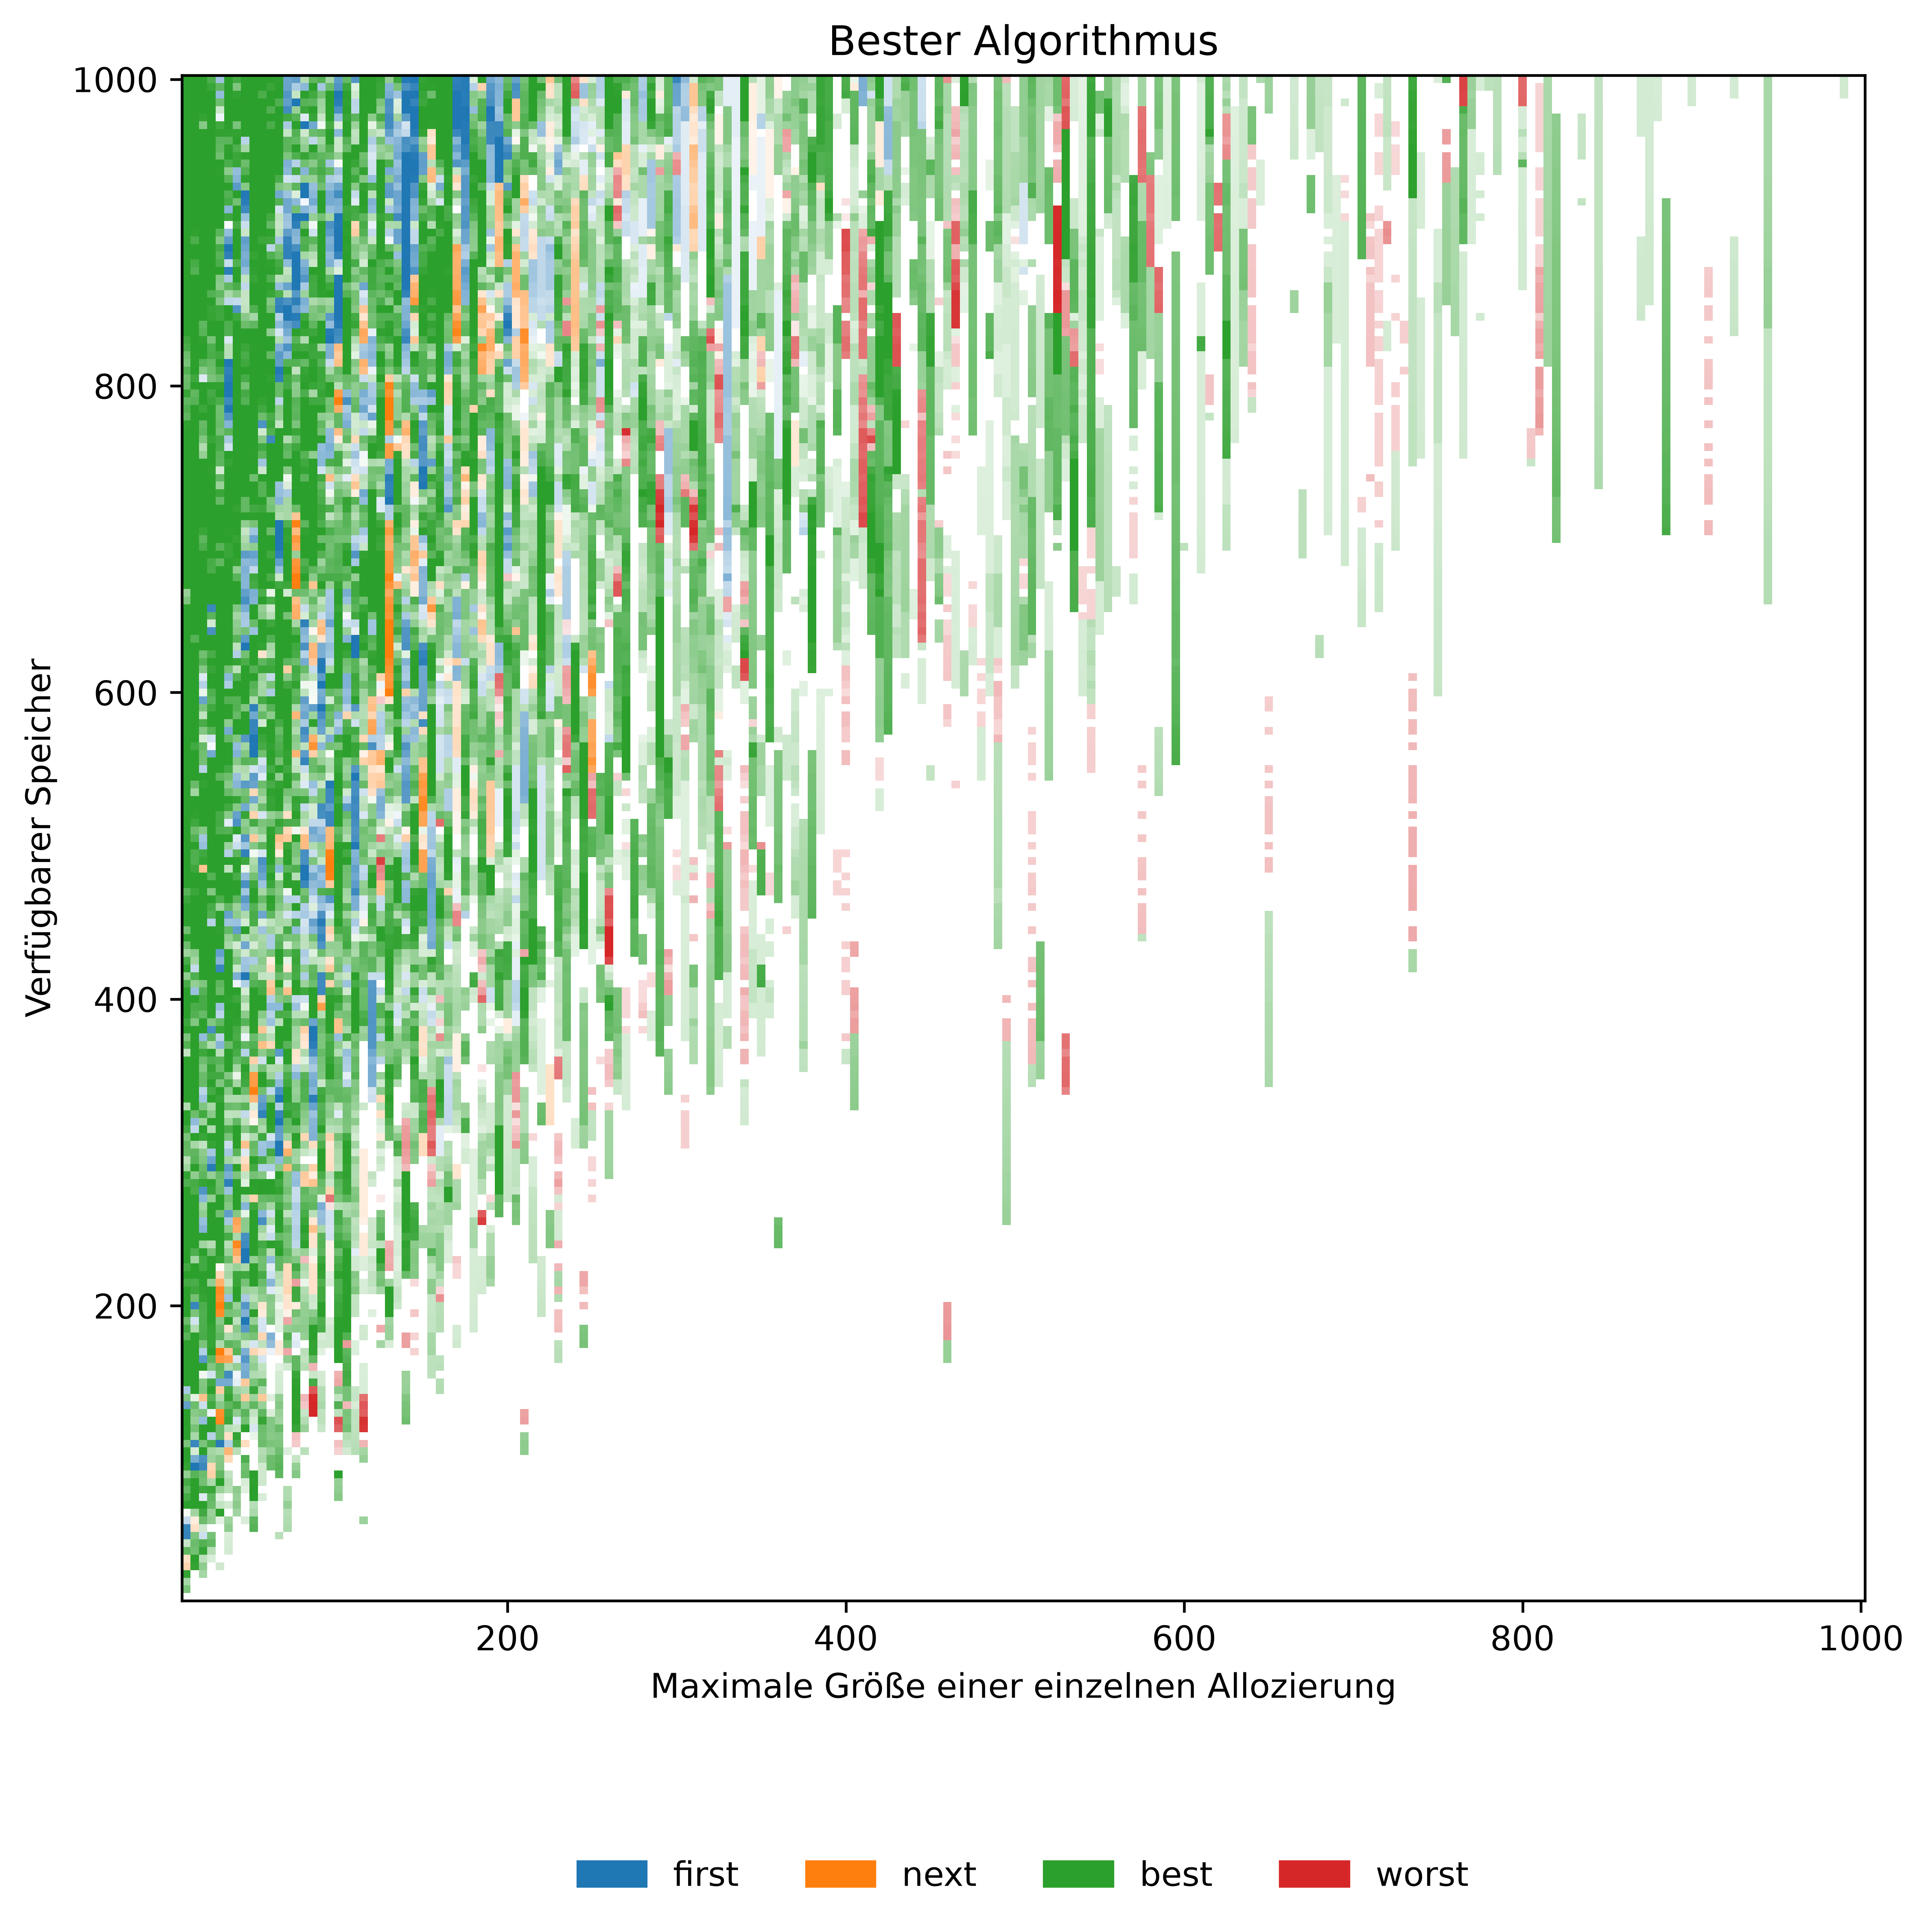
\includegraphics[width=.7\textwidth]{images/best_algo_2d.png}
  \caption{Vergleich Algorithmen als Heatmap.}
  \label{fig:best_algo}
\end{figure}

\begin{figure}
  \center
  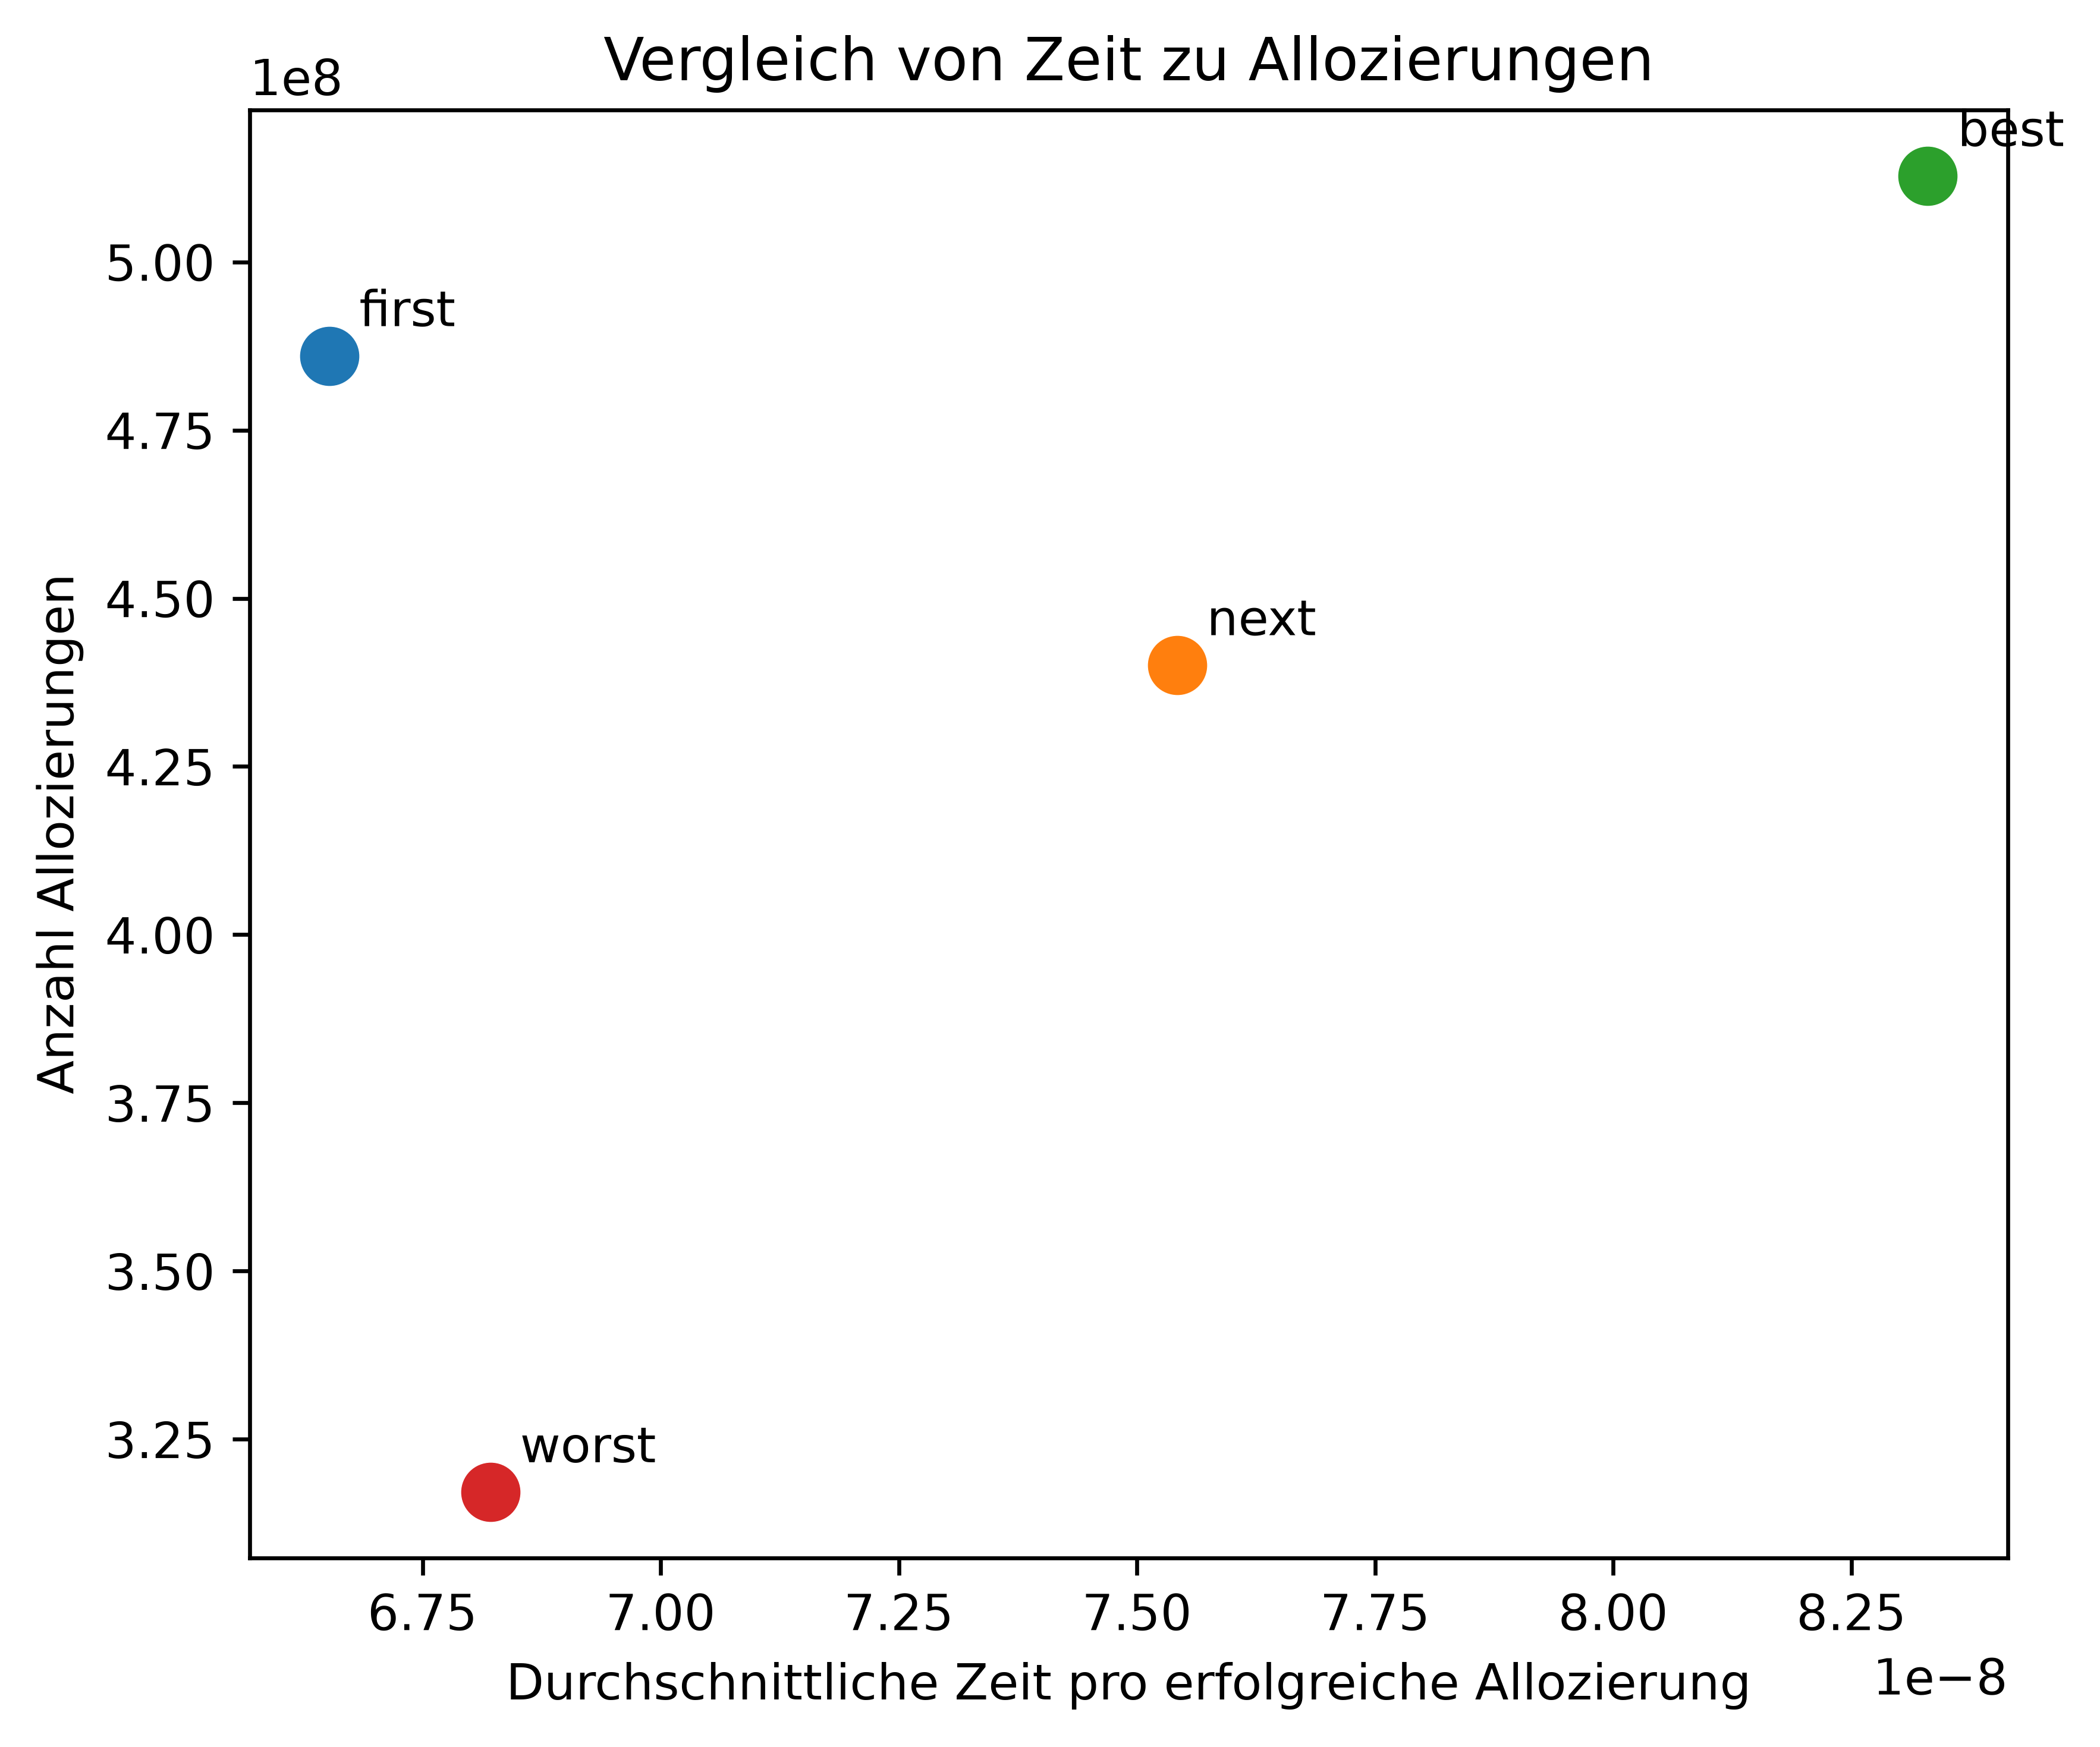
\includegraphics[width=.5\textwidth]{images/vergleich_zeit.png}
  \caption{Vergleich Algorithmen und deren benötigte Zeit.}
  \label{fig:time}
\end{figure}